\documentclass[letterpaper, 12pt]{article}
\usepackage{geometry}
\geometry{
    letterpaper,
    left=20mm,
    top=20mm,
    bottom=20mm
}
\usepackage{tocloft}
\usepackage{graphicx}
\usepackage{authblk}
\usepackage{amssymb}
\usepackage{lipsum}
\usepackage{float}
\usepackage{times}
\usepackage{amsmath}
\usepackage[format=plain,
            labelfont={bf,it},
            textfont=it]{caption}
\captionsetup{justification=raggedright,singlelinecheck=false}
\usepackage{ragged2e}
\usepackage{longtable}
\usepackage{comment}
\usepackage{setspace}
\usepackage{fancyhdr}
\usepackage{titlesec}
\usepackage[hyperindex,breaklinks]{hyperref}
\hypersetup{
    colorlinks=true,
    linkcolor=blue,
    filecolor=magenta,      
    urlcolor=blue
}
\usepackage[T1]{fontenc}
\usepackage{helvet}
\renewcommand{\familydefault}{\sfdefault}
\pagenumbering{gobble}
\usepackage[skip=10pt plus1pt, indent=40pt]{parskip}
\usepackage{orcidlink}
\usepackage{standalone}

\titlespacing*{\section}
{0pt}{1.5ex plus 1ex minus .2ex}{1.3ex plus .2ex}

\renewcommand\Authfont{\fontsize{12}{14.4}\selectfont}
\renewcommand\Affilfont{\fontsize{9}{10.8}\itshape}

\newcommand{\cosigpart}[1]{
  \addcontentsline{toc}{part}{#1}
}
\newcommand{\cosigsection}[1]{
  \section*{#1}
  \phantomsection % avoid warnings from hyperref about the anchor of a bookmark and its parent's
  \addcontentsline{toc}{section}{#1}
}
\begin{document}
\flushleft
\includegraphics[width=0.5\textwidth]{img/home/241017_final_logo_mockup.png}

\cosigsection{Example title}
\textit{Last updated: X Month 20XX}

This is a template for new guides to be added to COSIG.

\subsection*{Example section heading}

\begin{figure}[h!tbp]
    \centering
    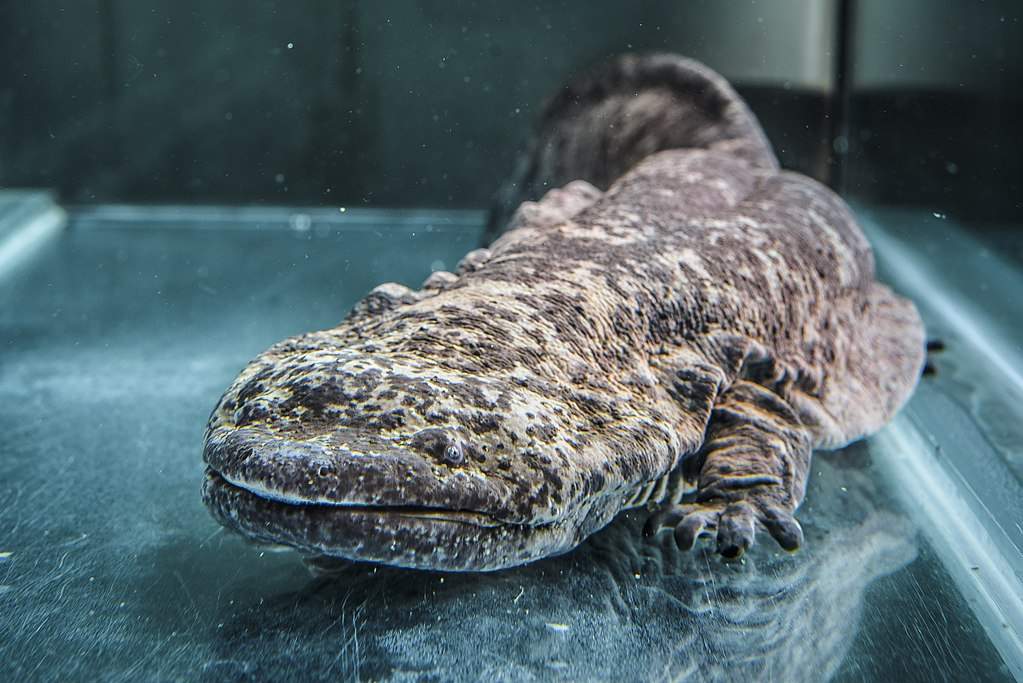
\includegraphics[width=0.8\textwidth]{img/home/chinese_giant_salamander.jpg}
    \caption*{Example of a figure. Image available \href{https://commons.wikimedia.org/wiki/File:Velemlok_\%C4\%8D\%C3\%ADnsk\%C3\%BD_zoo_praha_1.jpg}{here}.}
\end{figure}

\begin{itemize}
    \setlength\itemsep{-0.5em}
    \item bullet
    \item point
    \item list
\end{itemize}

\begin{enumerate}
    \setlength\itemsep{-0.5em}
    \item numbered
    \item list
\end{enumerate}

\pagebreak

\begin{center}
\begin{tabular}{|p{3.0cm}|p{3.0cm}|p{3.0cm}|}
\hline
     A & B & C\\ \hline\hline
     1 & 2 & 3\\\hline
     $\alpha$ & $\beta$ & $\gamma$\\ \hline
\end{tabular}
\end{center}

\begin{center}
\begin{tabular}{l|ccc}
& \multicolumn{3}{c}{predicted class} \\
true class & lemon & orange & tangerine \\
\hline
lemon & 1 & 1 & 0\\
orange & 0 & 1 & 2\\
tangerine & 0 & 0 & 1\\
\end{tabular}
\end{center}

If there is a large block of quoted text, use:

\begin{quote}
    \textit{Note that this text is in italics!}
\end{quote}

When linking out to articles using \verb|\href|, try to use the DOI instead of a link to the publisher site or PubMed page.

\end{document}